\chapter{PrePostTest}
\usetikzlibrary{quotes,angles,calc}
Which angle is bigger in each pair?

\begin{tikzpicture}[thick, scale= 2]
	\draw (0,0) -- (0:1);
	\draw (0,0) -- (80:1);
	\begin{scope}[shift={(2,0)}]
		\draw (0,0) -- (60:2);
		\draw (0,0) -- (20:2);
  \end{scope}
\end{tikzpicture}

\bigskip

\begin{tikzpicture}[thick, scale= 2]
	\draw (0,0) -- (45:1);
	\draw (0,0) -- (-45:1);
	\begin{scope}[shift={(2,0)}]
		\draw (0,0) -- (-45:1);
		\draw (0,0) -- (-135:1);
  \end{scope}
\end{tikzpicture}

\begin{tikzpicture}[thick, scale= 2]
	\draw (0,0) -- (60:1);
	\draw (0,0) -- (80:1);
	\begin{scope}[shift={(2,0)}]
		\draw (0,0) -- (40:1);
		\draw (0,0) -- (10:1);
  \end{scope}
\end{tikzpicture}

Find the missing measures of the angles (59 logo and geometry)

\begin{tikzpicture}
  \draw
  (3,-1) coordinate (a) node[right] {a}
  -- (0,0) coordinate (b) node[left] {b}
  -- (2,2) coordinate (c) node[above right] {c}
  pic["$\alpha$",draw=orange,<->,angle eccentricity=1.2,angle radius=1cm] {angle=a--b--c};
\end{tikzpicture}

\newcommand{\tikzAngleOfLine}{\tikz@AngleOfLine}                               
  \def\tikz@AngleOfLine(#1)(#2)#3{%                                            
  \pgfmathanglebetweenpoints{%                                                 
    \pgfpointanchor{#1}{center}}{%                                             
    \pgfpointanchor{#2}{center}}                                               
  \pgfmathsetmacro{#3}{\pgfmathresult}%                                        
  }                                                                            
\newcommand{\tikzMarkAngle}[3]{                                                
\tikzAngleOfLine#1#2{\AngleStart}                                              
\tikzAngleOfLine#1#3{\AngleEnd}                                                
\draw #1+(\AngleStart:0.15cm) arc (\AngleStart:\AngleEnd:0.15cm);              
}                                                                              

\begin{tikzpicture}[scale=4,line width=1pt]                                    
  \coordinate (A) at (0,0);                                                    
  \coordinate (B) at ($(A)+(90:1)$);                                                    
  \coordinate (C) at ($(B)+(-30:2)$);                                                
  \draw (A) -- (B) -- (C) -- cycle;                                            
	
  \tikzMarkAngle{(C)}{(B)}{(A)}   
	\node at ($(C)+(160:0.23)$) {?=\underline{\hspace{1cm}}};
	
	\tikzMarkAngle{(A)}{(B)}{(C)}
	\node at ($(A)+(45:0.23)$) {$90^\circ$};
	
	\tikzMarkAngle{(B)}{(A)}{(C)}           
	\node at ($(B)+(-60:0.23)$) {$60^\circ$};
\end{tikzpicture}  

\begin{tikzpicture}[scale=4,line width=1pt]                                    
  \coordinate (A) at (0,0);                                                    
  \coordinate (B) at ($(A)+(80:1)$);                                                    
  \coordinate (D) at ($(A)+(0:3)$);                                                
	\coordinate (C) at ($(D)+(100:1.5)$);
  \draw (A) -- (B) -- (C) -- (D) -- cycle;                                            
	
  \tikzMarkAngle{(A)}{(B)}{(D)}   
	
	\tikzMarkAngle{(C)}{(B)}{(D)}           
	
	\tikzMarkAngle{(D)}{(A)}{(C)}          
	
	\draw[shift={(B)}] (-100:0.15cm) arc (-100:10:0.15cm);
\end{tikzpicture}  

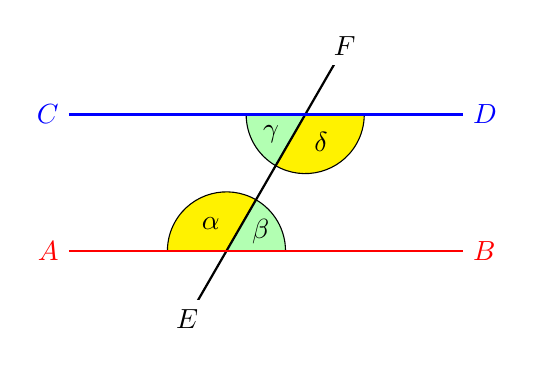
\begin{tikzpicture}
  \draw[fill=yellow] (0,0) -- (60:.75cm) arc (60:180:.75cm);
  \draw(120:0.4cm) node {$\alpha$};

  \draw[fill=green!30] (0,0) -- (right:.75cm) arc (0:60:.75cm);
  \draw(30:0.5cm) node {$\beta$};

  \begin{scope}[shift={(60:2cm)}]
    \draw[fill=green!30] (0,0) -- (180:.75cm) arc (180:240:.75cm);
    \draw (30:-0.5cm) node {$\gamma$};

    \draw[fill=yellow] (0,0) -- (240:.75cm) arc (240:360:.75cm);
    \draw (-60:0.4cm) node {$\delta$};
  \end{scope}

  \begin{scope}[thick]
    \draw (60:-1cm) node[fill=white] {$E$} -- (60:3cm) node[fill=white] {$F$};
    \draw[red]                   (-2,0) node[left] {$A$} -- (3,0) 
                                        node[right]{$B$};
    \draw[blue,shift={(60:2cm)}] (-3,0) node[left] {$C$} -- (2,0) 
                                        node[right]{$D$};
  \end{scope}
\end{tikzpicture}

Estimate the angles

\begin{tikzpicture}[scale=4,line width=1pt]                                    
  \coordinate (A) at (0,0);                                                    
  \coordinate (B) at ($(A)+(90:1)$);                                                    
  \coordinate (C) at ($(A)+(30:1)$);                                                
  \draw (A) -- (B);                                            
	\draw (A) -- (C);                                            
  \tikzMarkAngle{(A)}{(B)}{(C)}   
\end{tikzpicture}  

\begin{tikzpicture}[scale=4,line width=1pt]                                    
  \coordinate (A) at (0,0);                                                    
  \coordinate (B) at ($(A)+(90:1)$);                                                    
  \coordinate (C) at ($(A)+(0:1)$);                                                
  \draw (A) -- (B);                                            
	\draw (A) -- (C);                                            
  \tikzMarkAngle{(A)}{(B)}{(C)}   
\end{tikzpicture}  

\begin{tikzpicture}[scale=4,line width=1pt]                                    
  \coordinate (A) at (0,0);                                                    
  \coordinate (B) at ($(A)+(120:1)$);                                                    
  \coordinate (C) at ($(A)+(0:1)$);                                                
  \draw (A) -- (B);                                            
	\draw (A) -- (C);                                            
  \tikzMarkAngle{(A)}{(B)}{(C)}   
\end{tikzpicture}  

\begin{tikzpicture}[scale=4,line width=1pt]                                    
  \coordinate (A) at (0,0);                                                    
  \coordinate (B) at ($(A)+(-90:1)$);                                                    
  \coordinate (C) at ($(A)+(-135:1)$);                                                
  \draw (A) -- (B);                                            
	\draw (A) -- (C);                                            
  \tikzMarkAngle{(A)}{(B)}{(C)}   
\end{tikzpicture}  

\begin{tikzpicture}[scale=4,line width=1pt]                                    
  \coordinate (A) at (0,0);                                                    
  \coordinate (B) at ($(A)+(0:1)$);                                                    
  \coordinate (C) at ($(A)+(180:1)$);                                                
  \draw (A) -- (B);                                            
	\draw (A) -- (C);                                            
  \tikzMarkAngle{(A)}{(B)}{(C)}   
\end{tikzpicture}  

%parallelogram
\begin{tikzpicture}[scale=4,line width=1pt]                                    
  \coordinate (A) at (0,0);                                                    
  \coordinate (B) at (2,0);                                                    
  \coordinate (C) at ($(B)+(150:1)$);                                                
	\coordinate (D) at ($(A)+(150:1)$);                                                
  \draw (A) -- (B) -- (C) -- (D) -- cycle;                                            
	
  \tikzMarkAngle{(A)}{(B)}{(D)}   
	
	\tikzMarkAngle{(B)}{(A)}{(C)}
	
	\tikzMarkAngle{(C)}{(B)}{(D)}           
	\draw[shift={(D)}] (-30:0.15cm) arc (-30:0:0.15cm);      
\end{tikzpicture}  

\begin{tabularx}{\textwidth}{ |X|X| }
  \hline
  \begin{tikzpicture}[scale=4,line width=1pt]                                    
  \coordinate (A) at (0,0);                                                    
  \coordinate (B) at ($(A)+(-90:1)$);                                                    
  \coordinate (C) at ($(A)+(-135:1)$);                                                
  \draw (A) -- (B);                                            
	\draw (A) -- (C);                                            
  \tikzMarkAngle{(A)}{(B)}{(C)}   
\end{tikzpicture}  
	& 
item2
	
	
	\\
  \hline
  \square \hspace{0.5cm} 30^\circ \newline
\square \hspace{0.5cm} 45^\circ \newline
\square \hspace{0.5cm} 60^\circ \newline
\square \hspace{0.5cm} 90^\circ \newline
\square \hspace{0.5cm} 120^\circ \newline
\square \hspace{0.5cm} 150^\circ \newline
\square \hspace{0.5cm} 180^\circ 
 & 
item 2  \\
  \hline
\end{tabularx}

\begin{table}
    \begin{tabular}{ll}
    
		  \begin{tikzpicture}[scale=4,line width=1pt]                                    
  \coordinate (A) at (0,0);                                                    
  \coordinate (B) at ($(A)+(-90:1)$);                                                    
  \coordinate (C) at ($(A)+(-135:1)$);                                                
  \draw (A) -- (B);                                            
	\draw (A) -- (C);                                            
  \tikzMarkAngle{(A)}{(B)}{(C)}   
\end{tikzpicture}  
		
		
		& 
		  \square \hspace{0.5cm} 30^\circ \newline
\square \hspace{0.5cm} 45^\circ \newline
\square \hspace{0.5cm} 60^\circ \newline
\square \hspace{0.5cm} 90^\circ \newline
\square \hspace{0.5cm} 120^\circ \newline
\square \hspace{0.5cm} 150^\circ \newline
\square \hspace{0.5cm} 180^\circ 
		
		\\
    \end{tabular}
\end{table}


\square \hspace{0.5cm} 30^\circ \newline
\square \hspace{0.5cm} 45^\circ \newline
\square \hspace{0.5cm} 60^\circ \newline
\square \hspace{0.5cm} 90^\circ \newline
\square \hspace{0.5cm} 120^\circ \newline
\square \hspace{0.5cm} 150^\circ \newline
\square \hspace{0.5cm} 180^\circ